
% !TEX root = DesignDocument.tex

\chapter{The Data Encryption Standard}

In 1975 the National Bureau of Standards along with IBM and the National Security Agency released the first nationally standardized encryption algorithm.
This algorithm at the time called LUCIFER and eventually labeled DES was the national standard for 25 years until it was supplanted by the Advanced Encryption Standard in 2000.
DES still has historic and scholastic significance which is why two implementations of it are provided here.
The first is a simplified version and the second is a Full software implementation of DES.

\begin{figure}[ht]
\begin{center}
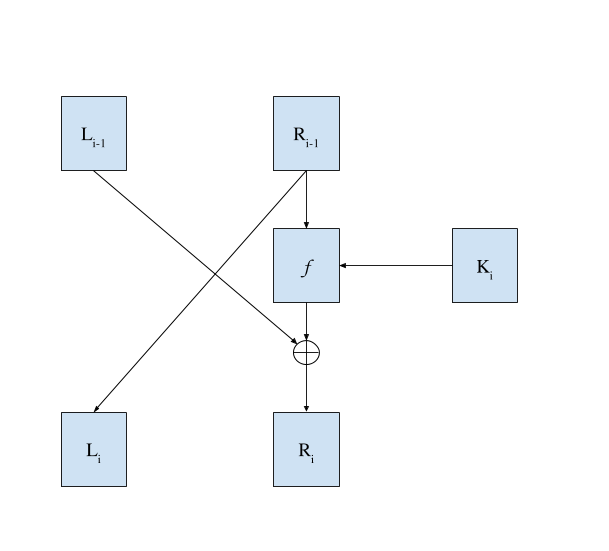
\includegraphics[width=0.75\textwidth]{./feistel}
\end{center}
\caption{Feistel system structure.}
\end{figure}

DES is a block cipher and a Feistel system. 
Named after Horst Feistel who was on the team which created LUCIFER.
Feistel systems tend to have many similar structures to them.
These include bit permutations, Multiple XORs and Substitution boxes.
The intent of any Feistel system is to create large changes in the plaintext with ever round.
However often as a consequence of their structure, encryption and decryption schemes are nearly identical.


\section{Simplified DES (SDES) }

The simplified version of the Data encryption standard ( SDES ) that is presented here uses four rounds and two substitution boxes to encrypt plaintext.
It is a block cypher just like DES, but instead of 64-bit block it uses 12-bit blocks. 
The key is also much smaller only 9-bits ( Although only 8-bits are used every round ).

\subsection{Encryption and Decryption}

\begin{figure}[ht]
\begin{center}
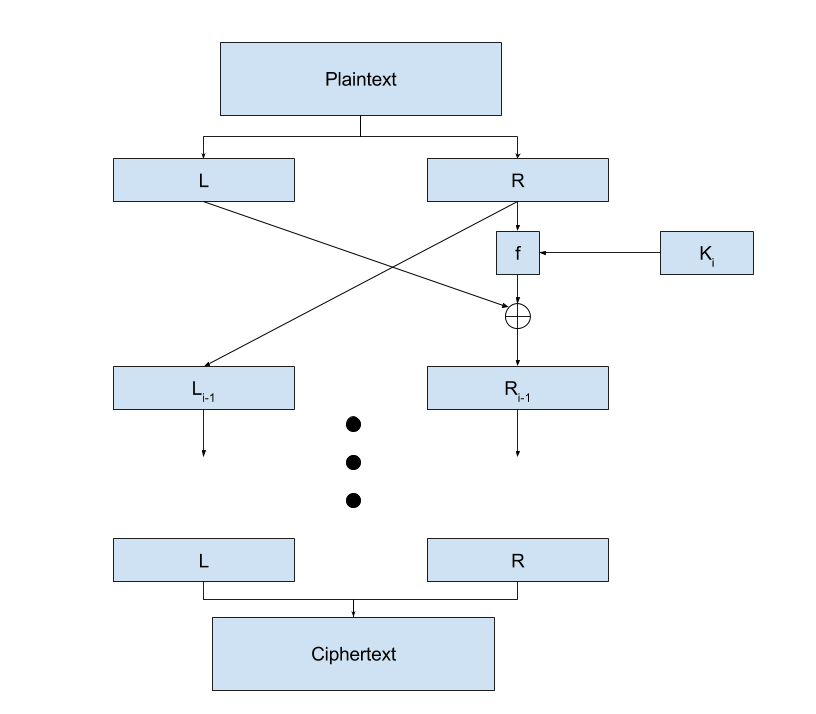
\includegraphics[width=0.75\textwidth]{./SDESflow}
\end{center}
\caption{Feistel system structure.}
\end{figure}

Unlike DES which has bit scrambling before the rounds and after, SDES simply splits the input text and begins the round.
A single round in SDES involves running the lower 6-bits through an expander to make it 8-bits.
Then the expanded input is run through the $f()$ function and XORing the result with the upper 6-bits of the plaintext.
That is then put into the lower 6-bits of the new input to the next round. The lower 6-bits from before the $f()$ function are then set as the upper 6-bits.

This algorithm is performed four times with the output from each becoming the input to the next system.

\subsection{$f()$ Function}
This function begins by expanding the input through the expander function.
The expanded input is then XORed with the key for that round.
That is then split into two 4-bit chunks which are are used to index into substitution boxes whose 3-bit outputs are concatenated into the output.

\subsection{ Substitution Boxes }
The Substitution box (Sbox) is an important part of any Feistel system.
Its purpose is provide a non-linear aspect to the encryption.
In SDES the 4-bit input is used to index into the 2x8 SBoxes, with the first bit choosing the row and the lower 3 bits choosing the column.

An important aspect of creating SBoxes are that small changes in the input should drastically change the output.
As such, any single bit change in the input the SBox also changes the output by at least one bit (2 bits in DES).

\begin{figure}[ht]
\begin{center}
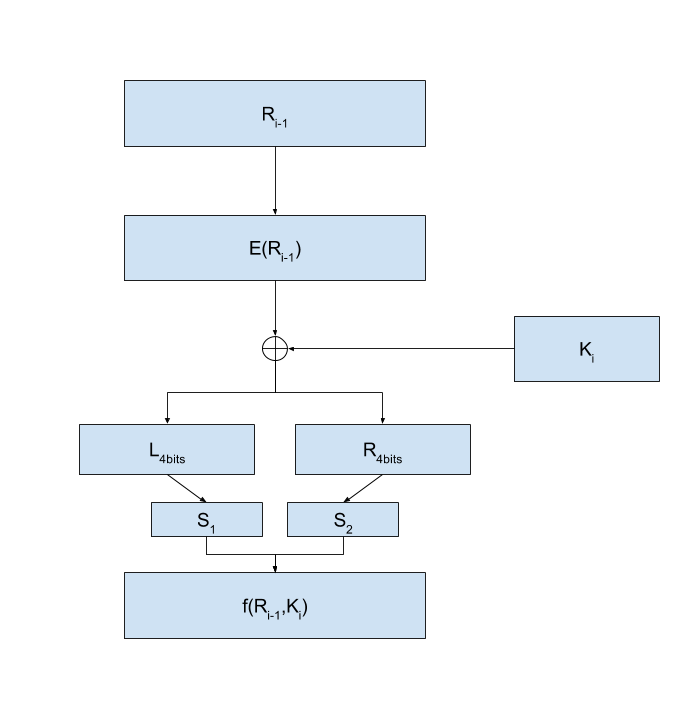
\includegraphics[width=0.5\textwidth]{./fFunc}
\end{center}
\caption{ One round of the SDES Feisel System.}
\end{figure}

\subsection{The Key Scheduler}

The final aspect of SDES is the key scheduler.
Being a much simplified version of DES the key scheduler is simply a rotating 9 bits.
Given a key of 9 bits a sliding window 8-bits wide slides down the key.
So the key looks like this through out the rounds:
\begin{align}
b_0b_1b_2b_3b_4b_5b_6b_7 \\
b_1b_2b_3b_4b_5b_6b_7b_8 \\
b_2b_3b_4b_5b_6b_7b_8b_1 \\
b_3b_4b_5b_6b_7b_8b_1b_2
\end{align}

\subsection{Implementation}

This package contains an implementation of SDES in 2 convenient programs.
To build this packages RSA implementation navigate to \textit{Cryptosuite/DES/Simple/} and run \textbf{make}, this will create \textit{DES\_unittest}, \textit{ encrypt} and \textit{decrypt}.

encrypt takes the key as a command line argument, and then begins reading from \textbf{stdin} since the block size is 12-bits and the reading must be done in 8-bit increments the program waits for 6 characters worth of input and then performs SDES on each block.
Due to system endianness at times the characters may be read incorrectly since the operation is being performed at a sub-byte level, this is corrected for.
Then the output is written to the buffer. This process is repeated until an \textbf{EOF} is reached.

decrypt works in much the same way, except it uses the keys in the reverse order. It does this easily since the function that performs a round also asks for a round number so it can do a key schedule.


\section{64-bit DES}

The full version of DES uses a 64-bit block size and the same size key*.
It has an increased number of Sboxes as well as bit permutations at nearly every step.
DES also uses 16 full rounds instead of 4.

\begin{figure}[ht]
\begin{center}
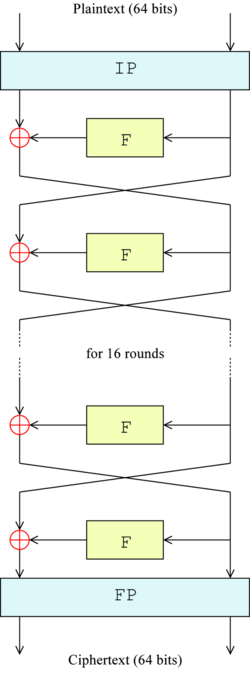
\includegraphics[width=0.5\textwidth]{./DESAlgo}
\end{center}
\caption{DES Algorithm Overview}
\end{figure}

\begin{figure}[ht]
\begin{center}
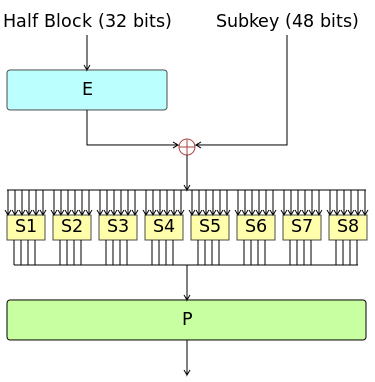
\includegraphics[width=0.4\textwidth]{./FFfunc}
\end{center}
\caption{DES Function $f(R_{i-1},K_i)$}
\end{figure}

\begin{figure}[ht]
\begin{center}
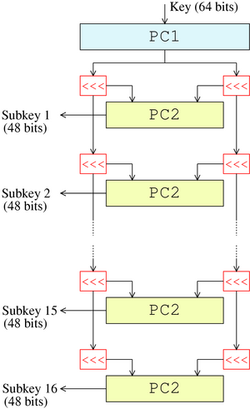
\includegraphics[width=0.3\textwidth]{./DESkey}
\end{center}
\caption{DES's key scheduler}
\end{figure}

\subsection{Encryption and Decryption}

The first thing done to any block of data is an initial permutation.
It is thought that these permutations provide no actual cryptographic significance, but did allow for easier loading on hardware in the 1970s
Other than this, the Full DES implementation functions much the same as SDES with the lower 32 bits of the plaintext being fed through the $f()$ function.
Finally the outputs are reversed a second time and run through an inverse permutation.
The result is the Ciphertext.

\subsection{$f()$ Function}
The round structure while being similar to DES is an order of magnitude more complex.
While they start similar with the 32-bit input becoming a 48-bit expanded output XORed with the key. 
After this the resultant 48-bits are split into 8 partitions which are fed into their 
respective SBoxes.
Then the result from that is  concatenated and run through another permutation before returning to be XORed with the upper 32 bits of the plaintext.

\subsection{ Substitution Boxes }

The Substitution boxes again function much the same as they do in SDES only they were chosen with much more care and are larger.
Most of the creation requirements are meant to discourage differential cryptoanalysis.

\begin{enumerate}
\item Each box has a 6 bit input and a 4 bit output.
\item They cannot be approximated by linear functions
\item Each row of the SBox must contain all numbers from 0 to 15
\item Any two inputs to any two S-boxes differing by 1 bit, must differ in 2 bits as outputs.
\item Any two inputs that differ in the first 2 bits but matching in the final two bit must ultimately be unequal.
\item Any 32 pairs of inputs given to any two boxes must not XOR to the same outputs more than 8 times.
\item The same is true for any 3 boxes.
\end{enumerate}

This is why DES is so resistant to differential analysis. 
In reality this kind of analysis is worthless on DES since the cost of differential analysis grows greater than brute force after 15 rounds.

\subsection{The Key Scheduler}

DES key scheduler is also steeped in permutation and obfuscation.
Initially the key is run through a permutation table to obtain 56-bits. 
You may recall the key actually has 64-bits but the remaining 8 are used as parity bits.
After each round the key is rotated either one or two bits to the left and permuted.
Then during each round a specific 48 bits bits are chosen to be XORed with the key.

During decryption and encryption it is possible and helpful to fully generate the key schedule beforehand.
This is especially true in decryption since the keys must be used in reverse order.


\subsection{Implementation}

This package contains an implementation of DES in 2 convenient programs.
To build this packages RSA implementation navigate to \textit{Cryptosuite/DES/Full/} and run \textbf{make}, this will create \textit{ encrypt} and \textit{decrypt}.

Unfortunately neither will function properly if run. 
Both are able to read input properly but as of writing the encrypt cannot give the proper output nor can decrypt undo encrypt.
The infrastructure is there but due to the obfuscating nature of the Feistel system debugging efforts have been unsuccessful.
